\section{Object and Event Selection}\label{sec:Zprime_HEEP}
Electron candidates are required to pass the so called ``HEEP'' (High Energy Electron Pairs) selection which is listed in Table \ref{tab:HEEPV70} followed by variables definition. In order to obtain well reconstructed electron candidates in tracker and ECAL sensitive regions, the candidates in the ECAL transition region (1.4442 < $|\eta|$ < 1.566) and beyond the $\eta$ coverage ($|\eta|$ > 2.5) of the tracker are therefore discarded.
After passing the HEEP selection the electrons are combined to form dielectron candidates.
If more than one dielectron candidate is found in the event, only the pair with the two largest electron \et is retained.
In addition, no charge requirement for dielectron candidates is asked and this is made to avoid efficiency losses at high mass for the main analysis.
Besides, at least one of the electron candidates has to be in barrel (events with both electron candidates in endcaps regions are rejected).
Events in data are required to satisfy the trigger selection described in Section \ref{sec:Zprime_trigger}.
MC events are weighted using turn on curves shown in Figures \ref{fig:L1_eff_2017}, \ref{fig:HLT_turnon_2016} and \ref{fig:HLT_turnon_2017} for considering the L1 and HLT effects.


\begin{table}[!h]
  \begin{center}
\smallskip\noindent
\resizebox{\linewidth}{!}{%
    \begin{tabular}{lll}
      \hline
      Variable                          & Barrel                             & Endcap                             \\
      \hline
      \multicolumn{3}{c}{Acceptance selections}\\
      \et                            & \et$>$ 35 GeV                    & \et$>$ 35 GeV                    \\
      $\eta$                            & $|\eta| < 1.4442$             & $1.566 < |\eta| < 2.5$        \\
      \hline
      \multicolumn{3}{c}{Identification selections}\\
      %\texttt{isEcalDriven}             & true                               & true                               \\
      $\Delta\eta_{in}^{seed}$          & $|\Delta\eta_{in}^{seed}| < 0.004$ & $|\Delta\eta_{in}^{seed}| < 0.006$ \\
      $\Delta\phi_{in}$                 & $|\Delta\phi_{in}| < 0.06$         & $|\Delta\phi_{in}| < 0.06$         \\
      $H/E$                             & $H/E < 1/E + 0.05$                 & $H/E < 5/E + 0.05$                 \\
      $\sigma_{i\eta i\eta}$            & -                                  & $\sigma_{i\eta i\eta} < 0.03$      \\
      $\frac{\EOnexFive}{\EFive}$ and $\frac{\ETwoxFive}{\EFive}$        & $\frac{\EOnexFive}{\EFive}>0.83$ or $\frac{\ETwoxFive}{\EFive}>0.94$ & -                              \\
      Inner layer lost hits             & lost hits $\le 1$                  & lost hits $\le 1$                    \\
      Impact parameter $d_{xy}$        & $|d_{xy}|<0.02$ cm                   & $|d_{xy}|<0.05$ cm                   \\
      isEcalDriven                     & true                                  & true                                  \\
      \hline
      \multicolumn{3}{c}{Isolation selections}\\
      \small{Calorimeter isolation} $Iso$                  & $Iso < 2 + 0.03\et[\mathrm{GeV}] + 0.28\rho$     & $Iso < 2.5 + 0.28\rho$ (\et<50 GeV) \\
                                        &                                    & else $Iso < 2.5 + 0.03(\et[\mathrm{GeV}]-50) + 0.28\rho$ \\
      Track \pt isolation $Isopt$       & $Isopt <$ 5 GeV                   & $Isopt <$ 5 GeV                   \\
      \hline
    \end{tabular}}
    \caption{The definitions of HEEP selection cuts \cite{HEEP_twiki}.}
    \label{tab:HEEPV70}
  \end{center}
\end{table}

The variables used in the HEEP definition are defined as follows \cite{HEEP_twiki}:
\begin{itemize}
\item[$\bullet$] \textbf{$\Delta\eta_{in}^{seed}$}:
 it is the difference in $\eta$ between the track position as measured in the inner layers, extrapolated to the interaction vertex and then extrapolated to the calorimeter and the $\eta$ of the supercluster's seed. The cut value in the barrel (0.004) is tighter than in the endcaps (0.006), because the tracker material budget is thicker in the endcaps and it reduces the precision on the position measurement.
\item[$\bullet$] \textbf{$\Delta\phi_{in}$}: it is the difference in $\phi$ between the track position as measured in the inner layers, extrapolated to the interaction vertex and then extrapolated to the calorimeter and the $\phi$ of the supercluster. Since there is a wider spread of the energy in $\phi$ with respect to $\eta$ due to photon emissions from bremsstrahlung processes of a electron, the distribution of $\Delta\phi_{in}$ is much broader than $\Delta\eta_{in}^{seed}$. Hence, The cut value of $\Delta\phi_{in}$ (0.06 in both barrel and endcap regions) is around ten times looser than for $\Delta\eta_{in}^{seed}$.

\item[$\bullet$] \textbf{\hoe}: it is a ratio of hadronic energy of the HCAL tower in a cone of radius 0.15 centred on the electron's position in the calorimeter to the electromagnetic energy of the electron's supercluster.

\item[$\bullet$] \textbf{\sieie}:
it is a measure of the spread in $\eta$ in units of crystals of the electrons energy in the $5\times5$ block centred on the seed crystal. It is computed as:
    $$\sieie = \sqrt{ \frac
      { \sum_{i \in 5\times5} \left( \eta_i - \bar \eta \right )^2 w_i
      } {\sum_{i \in 5\times5} w_i} }, ~~~~
    w_i = \max \left( 0, 4.7 + \log(E_i / E_{5\times5}) \right ).
    $$
\item[$\bullet$] \textbf{$\frac{\EOnexFive}{\EFive}$}: it is the ratio of the energy contained in the 1$\times$5 domino in $\eta\times\phi$ in the barrel ($x\times y$ in the endcaps) centered in $\phi$ on the seed crystal of the supercluster over the energy of the 5$\times$5 matrix centered on the same seed crystal.
\item[$\bullet$] \textbf{$\frac{\ETwoxFive}{\EFive}$}: it is the ratio of the energy contained in the most energetic 2$\times$5 domino in $\eta\times\phi$ in the barrel ($x\times y$ in the endcaps) centered in $\phi$ on the seed crystal of the supercluster over the energy of the 5$\times$5 matrix centered on the same seed crystal.
\item[$\bullet$] Inner layer lost hits : it is defined as the number of missing hits in the innermost layers of the tracker
(including the pixel) before the gsf track first hit. It is mainly designed to reject photons that convert into a pair of electrons in the tracker.
\item[$\bullet$] Impact parameter $d_{xy}$: it is the closest distance (in the transverse plane) between the primary vertex and the track of the gsf electron candidate. The distribution is wider in the endcaps due to the poorer resolution on the track momentum in that region. Similarly to the missing hit cut, the $d_{xy}$ cut is mainly useful to reject converted photons.
\item[$\bullet$] isEcalDriven : electrons can be ecal driven (found using egamma techniques) or tracker driven (found using particle flow algorithm). Tracker driven is useful for low energy electrons, while it is not useful or validated for high energy electrons. Hence we require that the electron be ecal driven.
\item[$\bullet$] ECAL isolation: it is defined as the scalar sum of the transverse energy of all the ECAL crystals with \et$>$
80 MeV in the barrel (\et$>$ 100 MeV in the endcaps) in a cone of $\Delta R$ = 0.3
centered on the gsf electron candidate position in the calorimeter, excluding those
in an inner cone of radius 3 crystals and those in a $|\eta|$ strip of total width of 3 crystals (see left side of Figure \ref{iso_pic}).
The inner cone veto removes the electron energy from the sum whereas the $|\eta|$ strip removes the energy from the bremsstrahlung photons.
\item[$\bullet$] { HCAL isolation: it is defined as the sum of transverse energy collected by all the towers
of the first layer of the HCAL in a cone of $\Delta R$ = 0.3 centered on the gsf electron
candidate position in the calorimeter, excluding the towers in a cone of $\Delta R$ = 0.15 (see right side of Figure \ref{iso_pic}).
\begin{figure}[!htbp]
\begin{center}
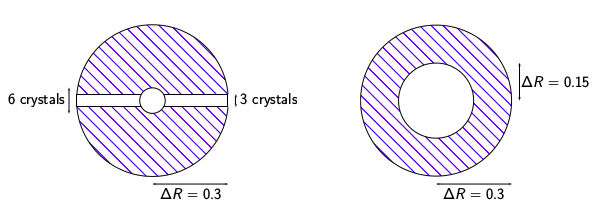
\includegraphics[width=0.8\textwidth]{figures/Zprime/iso.png}
\end{center}
\caption{Definition of the regions used to compute the ECAL (left) and HCAL (right) isolation.}
\label{iso_pic}
\end{figure}}

\item[$\bullet$] Calorimeter isolation $Iso$: it is sum of the ECAL isolation and the HCAL isolation (defined in the previous points). The variable is strongly dependent on the electron energy and tends to increase for high \et~electrons due to the extension of the shower. A cut value of the
form $Iso < a + b\cdot E_T$ is therefore applied.
\item[$\bullet$] Track \pt isolation $Isopt$: it is defined as the sum of the \pt of all the reconstructed
tracks between an inner and outer cone around the gsf electron. The $\Delta R$ for the inner cone is 0.04 and it is 0.3 for the outer cone.
Besides, only tracks having \pt > 700 MeV and $|\Delta z|$ with the gsf electron track $<$ 0.2 cm are considered, where z is the minimum distance of
the track to the nominal interaction point (0,0,0).
%The inner cone veto is present
%to remove duplicate tracks associated to the electron as well as tracks from converted
%bremsstrahlung photons. This variable substitutes the default tracker isolation variable in the gsf electron, for which the efficiency has a large pile-up dependence starting at $\et\sim100$~GeV, due to a misbehaviour of the reconstruction software that allows many low quality tracks to enter the isolation cone.  The track isolation variable has then been redefined introducing ad-hoc ``high purity'' requirements which removed most of the problematic tracks that introduced the pile-up dependance of this variable.
\end{itemize}
